\section{Structure}

At the very beginning of the development stage of this project, only one activity was used. The game launched directly into the game field, which was a canvas showing a bitmap image representing the ground on the game field. This worked well while experimenting with Android graphics. However, when menu development started a few weeks later, it was clear that more activities would be needed. A set of activities were created, everyone of them representing a different screen in the game.
 
The first activity being created is called SplashActivity. This is used only to display a splash screen for a few seconds. When the splash screen has been shown for those few seconds a new activity called Menu is created. The SplashActivity is then finished and removed from the activity stack. The Menu activity is not finished every time a menu item is clicked. Instead it remains on the activity stack, waiting to be shown after overlying activities are closed.

Four different activities can be started from the main menu: MenuGame, MenuHelp, MenuOptions and MenuCredits. These activities, together with the activity Menu, are the foundation of the game. The following chart visualizes the flow between different activities:

%-----
%- Image code structure
%-----
\begin{figure}[here]
\begin{center}
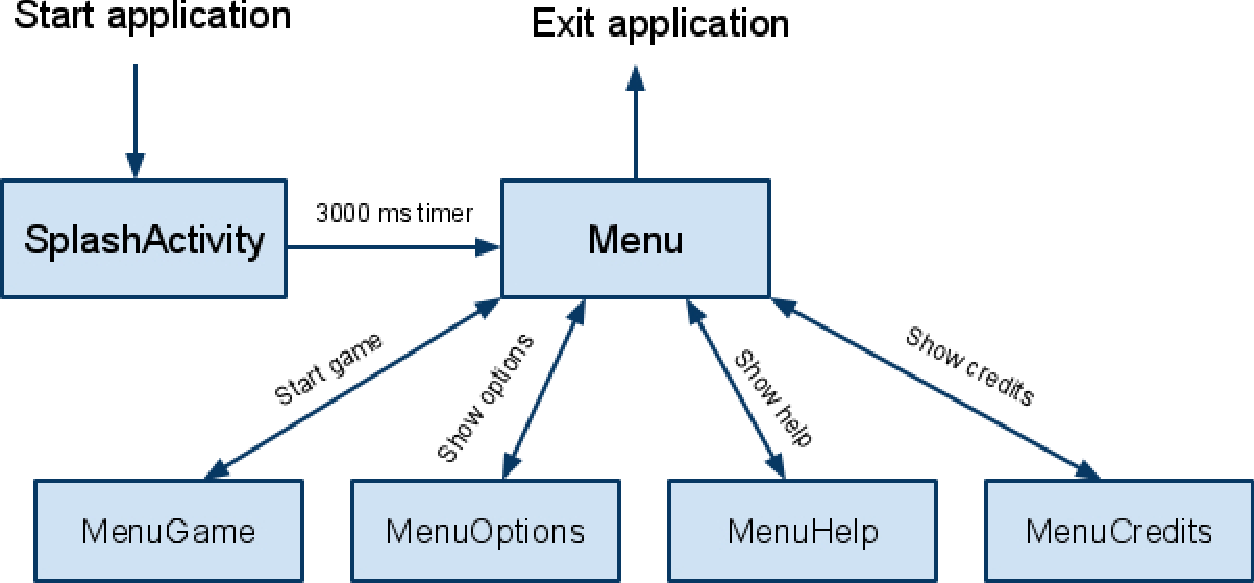
\includegraphics[scale=0.6]{pics/chapters/chapter4/codestructure}
\end{center}
\caption{Flowchart of activities in Eskimo Tower Defense}
\label{fig:codestructureActivities}
\end{figure}
%-----

Arrows in the flowchart above (figure ~\ref{fig:codestructureActivities}) indicate a transition between activities. All transitions except the one between SplashActivity and Menu are initiated by user actions, using in-game menu buttons. All navigation is done through in-game menus to give the user a more immersive experience.

The actual game is launched from the MenuGame activity. Two different view classes are used to display either the game field or the progression route map. Originally, only the game field View was shown in MenuGame. The progression route map was implemented at a later stage of development, and the idea of changing the View of MenuGame seemed like the most simple solution. With this solution the transition from the progression route map to the game field is performed by the different Views themselves (e.g when a track is started from the progression route map, the game field View is set as the visible View in MenuGame).

Not only Activity and View classes exist in the implementation of the game. When the View classes are created, a thread is also created for each View class. These threads continuously update the Views with regards to updating states and sound, and drawing whatever the View should display. 

The classes MobFactory, Path and Highscore are used to translate XML-files containing information about different tracks, to data stored in lists and arrays. This data is later read from other classes, such as GameView and GameModel.
 
After selecting "Start" from the main menus and selecting a track on the progression map, the game is started. The game is managed and drawn by the GameView class. This class handles graphics, sound, the game thread, user input, sensor-initiated events like the ones originating from the accelerometer and the different game states (PAUSED, RUNNING, GAMEOVER, WIN).

GameView does not contain any data about the objects' states in the game. It only contains a reference to GameModel which keeps track of all the data related to current states of the objects in the game. The GameView's task is to translate the data of the game into bitmaps drawn onto the screen and handle the user's input. 

In the constructor, the GameView initializes the GameThread class. This class is a thread that runs during the game. It constantly invokes the updateModel(), updateSounds() and onDraw() methods in GameModel. This updates the GameModel and the sound states, and draws the screen according to the data in GameModel. The GameThread also includes methods for handling the thread itself, e.g. a method to terminate the thread when exiting the game.

%--------------------------
%- Code snippet GameThread
%--------------------------
\begin{figure}[htb]

\begin{small}
\verbatiminput{code/GameThread.java}
\end{small}

\caption{Caption for GameThread}
\label{fig:codeExGameThread}
\end{figure}
%--------------------------

The code above (figure ~\ref{fig:codeExGameThread}) is placed in the run() method of the GameThread. The while loop is run as long as mRunThread is true, which it is as long as the game is running. The three method calls updateModel(), updateSounds() and onDraw() are placed inside a synchronized statement. This blocks the rest of the program so there is no interference from the user input or other threads while a frame of the game is calculated and drawn to the screen. 

The function of updateModel() is to update the model. The model is represented by the class GameModel that contains a list of all the objects on the screen, the player statistics, the path and some other properties of the game. The updateModel() method does all the calculation and algorithms that make the game work. It updates the positions of all units on the screen, creates new objects and sets the score according to what happens. 

The GameView contains an extra initializing method called startTrack(), which is called from the constructor of GameView. Since the track can be restarted from within the game there must be a method other than the constructor to reset all values, so the game can be played again. If all this code would have been placed in the constructor, the game would have to reload the entire GameView to restart, now it only has to call startTrack().